% !TeX root = paper.tex
\section{Experiment: Elementary Perceptual Tasks}

Cleveland and McGill describe the mapping of graphical elements to quantitative variables as \emph{elementary perceptual tasks} and introduce a list of ten different encodings in their paper~\cite{cleveland_mcgill,cleveland1985graphical}. These tasks are the low-level building blocks for information visualizations and encode quantities. Cleveland and McGill did not explicitly test human perception of single instances of these encodings. However, we test how each classifier measures encoded values using the elementary perceptual tasks and create visualizations of these tasks as rasterized images with different parametrizations (Table~\ref{tab:encoding_parameters}).

\subsection{Parametrizations}
\label{sec:parametrizations}
We generate multiple parameterizations for each elementary perceptual task and sequentially increase the number of parameters (Table~\ref{tab:encoding_parameters}). For instance, for \emph{Position Common Scale} we first only vary the $y$-position which yields just $60$ different parameters. We then include translation along the x-axis with a significant increase in variability. We then also add a variable spot size. This results in more complex datasets depending on the increase of variability. Table~\ref{tab:encoding_parameters} shows the different settings. It is important to consider this variability when evaluating different classifiers with individual trainable parameters (Table~\ref{tab:parameters}). In theory, classifiers can memorize the images if the data set has a low variability. We also counteract such behavior by adding noise.

%\begin{figure}[t]
%	  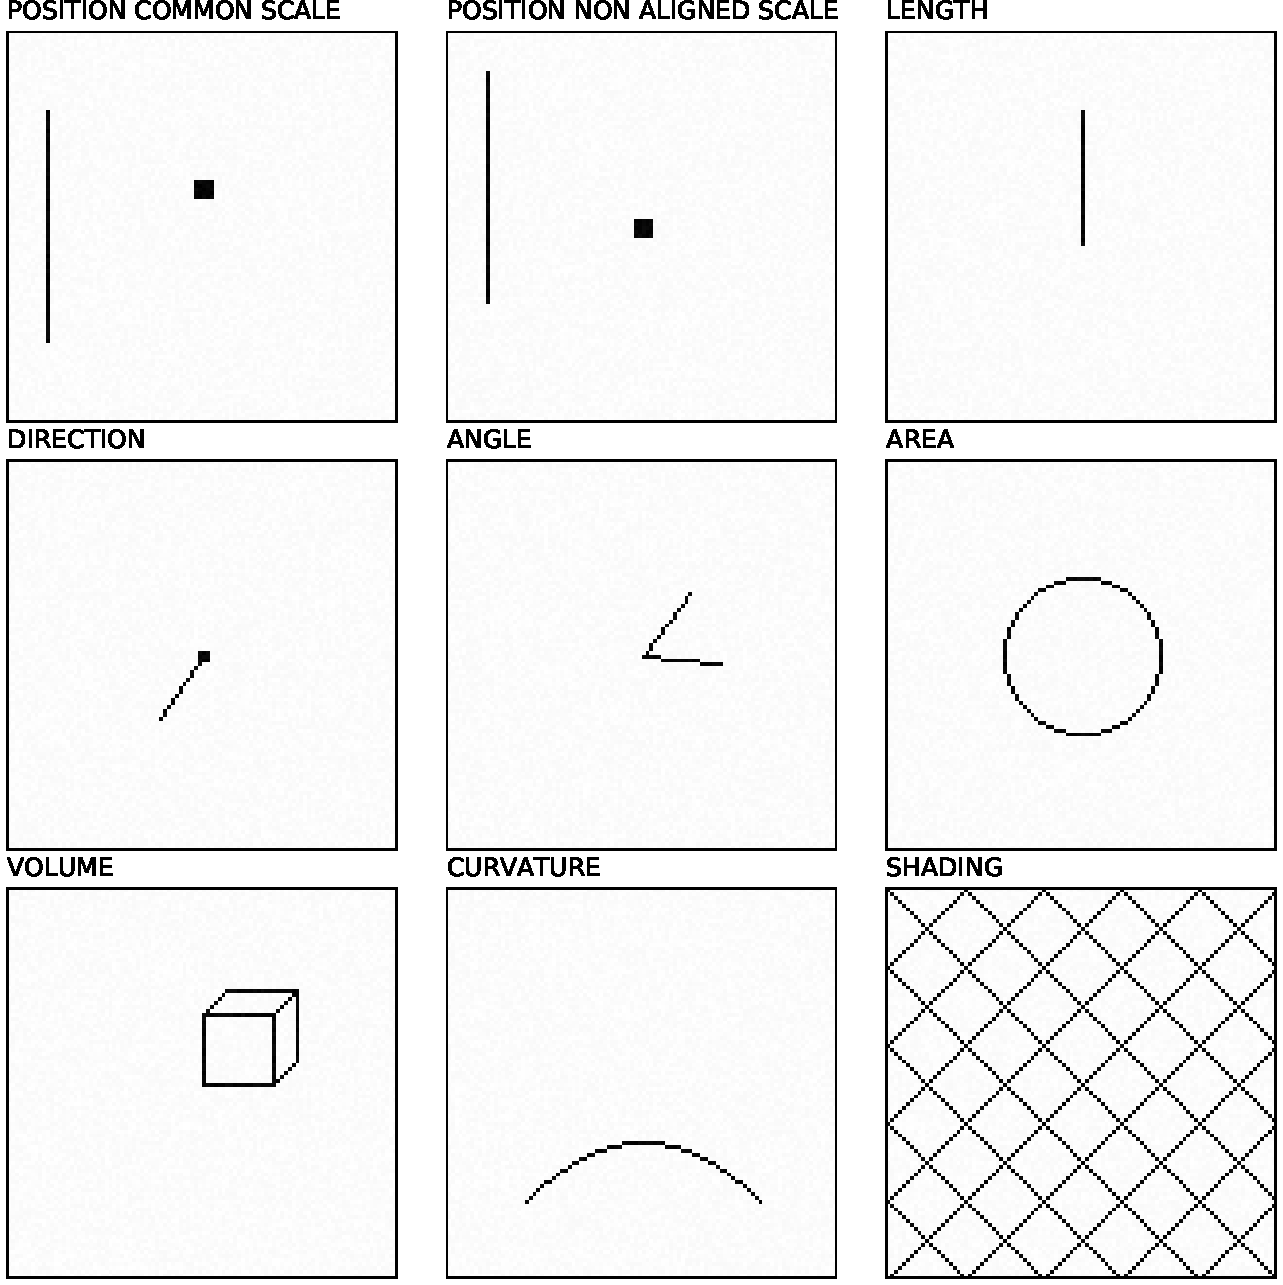
\includegraphics[width=\linewidth]{figure1_overview.pdf}
%  \caption{\textbf{Elementary Perceptual Tasks.} Rasterized visualizations of the elementary perceptual tasks as defined by Cleveland and McGill~\cite{cleveland_mcgill} (color saturation excluded). We vary the parameters of each perceptual task and then assess the interpretability of feed-forward neural networks.}
%	\label{fig:elementary_perceptual_tasks}
%\end{figure}



\begin{table}[!ht]
\centering
\caption{\textbf{Elementary Perceptual Tasks.} Rasterized visualizations of the elementary perceptual tasks as defined by Cleveland and McGill~\cite{cleveland_mcgill} (color saturation excluded). We sequentially increase the number of parameters (e.g. by adding translation) for every task. This introduces variability and creates increasingly more complex datasets.}
\resizebox{\linewidth}{!}{
\begin{tabular}{lllr}
	\toprule
	\multicolumn{2}{l}{Elementary Perceptual Task} & ~ & Permutations\\
	\midrule
	\raisebox{-.85\height}{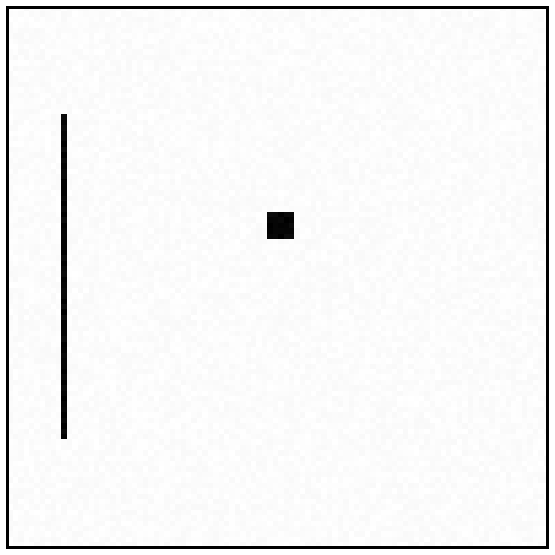
\includegraphics[width=.5in]{position_common_scale.pdf}} & \makecell[tl]{\emph{Position Common Scale}\\~~~Position Y\\~~~+ Position X \\~~~+ Spot Size \\} &~& \makecell[tr]{~\\ $60$ \\ $3,600$ \\ $216,00$}\\

	\midrule
	\raisebox{-.85\height}{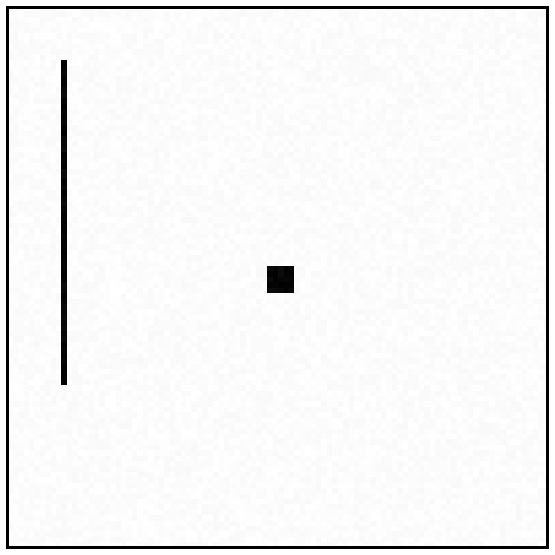
\includegraphics[width=.5in]{position_non_aligned_scale.pdf}} & \makecell[tl]{\emph{Position Non-Aligned Scale}\\~~~Position Y\\~~~+ Position X \\~~~+ Spot Size \\} &~& \makecell[tr]{~\\ $600$ \\ $36,000$ \\ $216,000$}\\

	\midrule
	\raisebox{-.95\height}{
\includegraphics[width=.5in]{length.pdf}} & \makecell[tl]{\emph{Length}\\~~~Length\\~~~+ Position Y \\~~~+ Position X \\~~~+ Width} &~& \makecell[tr]{ ~\\$60$ \\ $2,400$ \\ $144,000$\\$864,000$}\\

	\midrule
	\raisebox{-.85\height}{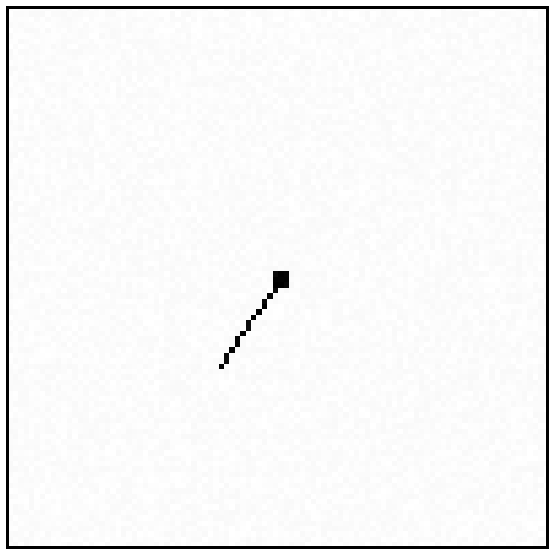
\includegraphics[width=.5in]{direction.pdf}} & \makecell[tl]{\emph{Direction}\\~~~Angle\\~~~+ Position Y \\~~~+ Position X} &~& \makecell[tr]{ ~\\$360$ \\ $21,600$ \\ $1,296,000$}\\

	\midrule
	\raisebox{-.85\height}{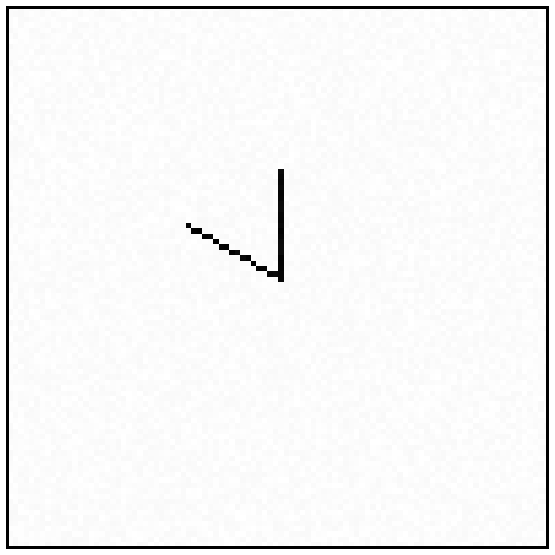
\includegraphics[width=.5in]{angle.pdf}} & \makecell[tl]{\emph{Angle}\\~~~Angle\\~~~+ Position Y \\~~~+ Position X} &~& \makecell[tr]{ ~\\$90$ \\ $5,400$ \\ $324,000$}\\

	\midrule
	\raisebox{-.85\height}{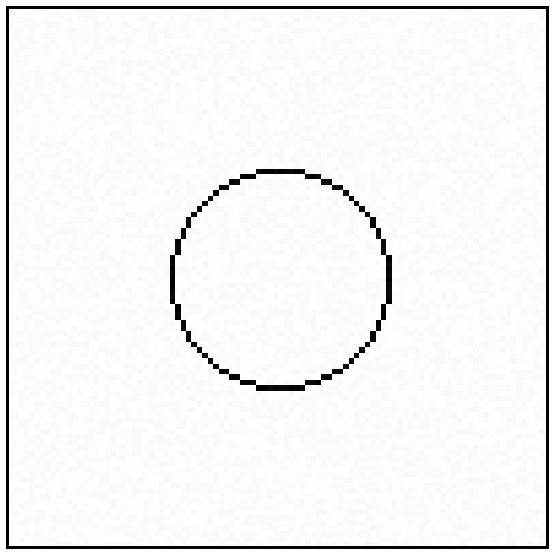
\includegraphics[width=.5in]{area.pdf}} & \makecell[tl]{\emph{Area}\\~~~Radius\\~~~+ Position Y \\~~~+ Position X} &~& \makecell[tr]{ ~\\$40$ \\ $800$ \\ $16,000$}\\

	\midrule
	\raisebox{-.85\height}{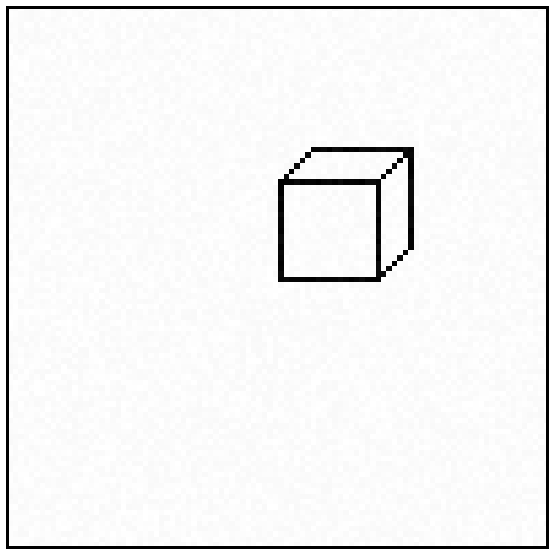
\includegraphics[width=.5in]{volume.pdf}} & \makecell[tl]{\emph{Volume}\\~~~Cube Sidelength\\~~~+ Position Y \\~~~+ Position X} &~& \makecell[tr]{ ~\\$20$ \\ $400$ \\ $8,000$}\\
	
	\midrule
	\raisebox{-.85\height}{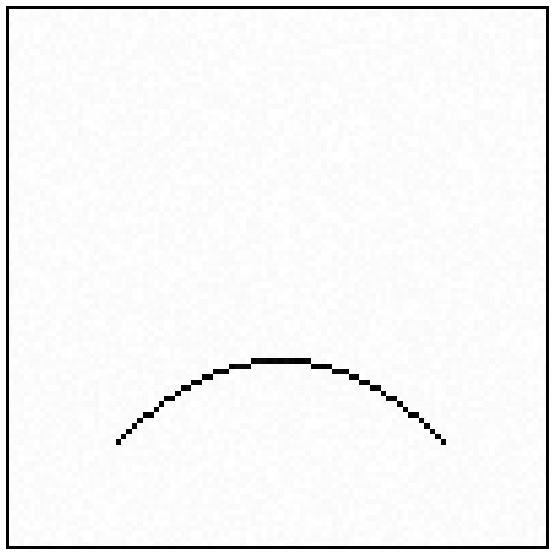
\includegraphics[width=.5in]{curvature.pdf}} & \makecell[tl]{\emph{Curvature}\\~~~Midpoint Curvature\\~~~+ Position Y \\~~~+ Position X} &~& \makecell[tr]{ ~\\$80$ \\ $1,600$ \\ $64,000$}\\	

	\midrule
	\raisebox{-.85\height}{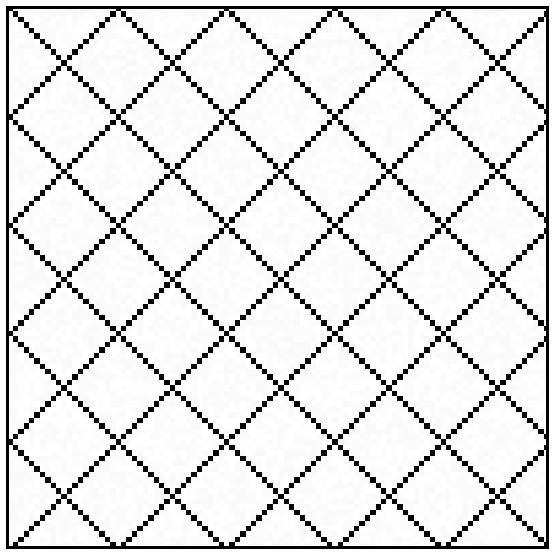
\includegraphics[width=.5in]{shading.pdf}} & \makecell[tl]{\emph{Shading}\\~~~Density\\~~~+ Position Y \\~~~+ Position X} &~& \makecell[tr]{ ~\\$100$ \\ $2,000$ \\ $40,000$}\\	
%	
	\bottomrule
\end{tabular}
}
\label{tab:encoding_parameters}
\end{table}



%
\subsection{Hypotheses}

We proposed four hypotheses entering the elementary perceptual task experiment:

\begin{itemize}
	\item \textbf{H1.1} \textbf{Our convolutional neural networks are able to regress quantitative variables from graphical elements.} We parametrize different visual encodings (Table~\ref{tab:encoding_parameters}) and test whether the CNNs can measure them with an accuracy similar to humans.
	\item \textbf{H1.2} \textbf{Computed perceptual performance is dependent on network architexture.} We evaluate multiple regressors with different numbers of trainable parameters. A more complex network (with a higher number of parameters) might perform better on elementary perceptual tasks.
	\item \textbf{H1.3} \textbf{Some visual encodings are better than others for computations.} Cleveland and McGill order the elementary perceptual tasks by accuracy. We investigate whether this order is also relevant for computing graphical perception.
	\item \textbf{H1.4} \textbf{Networks trained on perceptual tasks can generalize to more or less complex variations of the same task.} Recent research suggests that convolutional neural networks are able to generalize by interpolating between different datapoints. While the underlying reasons are mainly yet unknown, this property allows them to perform on variations of a similar perceptual task. We create visual representations of the elementary perceptual tasks with different variability (Table~\ref{tab:encoding_parameters}). We suspect that such variations are not a problem for successfully regressing the quantitative variables and that the networks are able to generalize.
\end{itemize}

%	
%	We suspect that CNNs are able to 'learn` absolute quantities encoded using low-level visual 
%	
%	While much simpler models than their biological pendant, convolutional neural networks are heavily influenced by our biological knowledge of the visual system. Such classifiers therefor follow the same principles as human perception.


\subsection{Results}

The results of the elementary perceptual tasks experiment demonstrates that our networks are able to measure visually encoded quantities using low-level building blocks (Fig.~\ref{tab:figure1_results}). While the performance varies for the different encodings, we observe for all networks performance similar to the measured human performance by Cleveland and McGill~\cite{cleveland1985graphical}. These results confirm our initial hypotheses.
\\~\\
\noindent{\textbf{Accuracy.}} We report the average error across all tasks for our networks as \textit{MLAE}: 
$2.943$ ($SD=0.857$) for the multilayer perceptron, 
for LeNet $2.125$ ($SD=0.38$), 
VGG19 on ImageNet $0.979$ ($SD=0.581$), 
for VGG19 trained from scratch $0.404$ ($SD=0.407$), 
Xception on ImageNet $1.627$ ($SD=0.462$), 
and for the re-trained Xception $1.504$ ($SD=0.493$). The average error for all classifiers is \textit{MLAE}$=1.597$ ($SD=0.394$) and \textit{MAE}=$2.89$ ($SD=0.848$). VGG19 trained from scratch reaches the best performance overall.
These values are in the same ballpark as the range of $8-14\%$ error (approx. MLAE=$3$) for a similar experiment by Cleveland and McGill testing human estimation of relations between elementary perceptual tasks~\cite{cleveland1985graphical}. We therefor carefully confirm that our networks are able to regress the graphical elements to quantities within a reasonable range of error and \textbf{accept H1.1}.
\\~\\
\noindent{\textbf{Regressor Complexity.}} The performance varies not only across different visual encodings but also very much across the different network architectures. We compare the average regression performances for our networks and report the effect of the regressor as statistical significant ($F_{5,48}=20.392,p<0.01$). Post hoc comparisons show that the differences between LeNet and the VGG19 network, independent of the used weights, are significant ($t_48=4.674,p<0.01$). VGG19 from scratch and Xception (both versions) are significant, from scratch ($t_48=4.87,p<0.01$) and for imagenet weights($t_48=5.621,p<0.01$). However, differences between LeNet and both Xception networks are not significant. In any case, the variation of results also visually inspectable in Fig.~\ref{fig:figure1_results} shows the variation of performance of the different networks. We therefor \textbf{partially accept H1.2}.
\\~\\
\noindent{\textbf{Ranking of Visual Encodings.}} Cleveland and McGill provide an ordering of elementary visual encodings based on theoretical arguments and experimental results. We re-create their ranking with MLAE values of our networks in Table~\ref{tab:ranking}. The rankings differ between the different networks and Cleveland and McGill's version. However, the ranking between networks using imagenet weights is identical. Since such a ranking see,s to heavily depend on the used regressor, the weights, and the initialization, we do not think a generalized ranking can be created and \textbf{reject H1.3}.

\begin{table}[!ht]
\centering
\caption{\textbf{Ranking of Elementary Perceptual Tasks.} We create a ranking of the elementary perceptual tasks for all of our networks. We report midmean logistic absolute errors (MLAE) for each network averaged across multiple runs on the most complex parametrization of the individual stimuli. The VGG19 network performs best compared on all tasks. For human performance, we report the ranking of Cleveland and McGill~\cite{cleveland_mcgill}. The VGG19 * and Xception * networks use ImageNet weights and yield identical rankings.}
\resizebox{\linewidth}{!}{
\begin{tabular}{cllllll}
\toprule
Human & MLP & LeNet & VGG19 * & \textbf{VGG19} & Xception * & Xception \\
\midrule
\multicolumn{7}{l}{\emph{Position Common Scale}} \\
1. & 7. (3.84) & 2. (1.36) & 5. (1.02) & \textbf{3.} (-0.04) & 5. (1.65) & 1. (1.04)\\
\multicolumn{7}{l}{\emph{Position Non aligned Scale}} \\
2. & 6. (3.61) & 1. (1.35) & 6. (1.09) & \textbf{5.} (0.26) & 6. (1.71) & 2. (1.06)\\
\multicolumn{7}{l}{\emph{Length}} \\
3. & 1. (1.99) & 8. (3.19) & 4. (0.87) & \textbf{2.} (-0.14) & 4. (1.59) & 3. (1.11) \\
\multicolumn{7}{l}{\emph{Direction}} \\
3. & 9. (4.65) & 7. (3.07) & 9. (2.84) & \textbf{8.} (0.92) & 9. (3.46) & 6. (1.57) \\
\multicolumn{7}{l}{\emph{Angle}} \\
3. & 8. (4.61) & 9. (3.33) & 8. (2.31) & \textbf{9.} (0.99) & 8. (2.60) & 7. (1.72) \\
\multicolumn{7}{l}{\emph{Area}} \\
4. & 2. (2.01) & 5. (2.21) & 1. (0.49) & \textbf{1.} (-0.17) & 1. (0.80) & 5. (1.38) \\
\multicolumn{7}{l}{\emph{Volume}} \\
5. & 4. (2.38) & 4. (1.91) & 7. (1.16) & \textbf{7.} (0.87) & 7. (2.03) & 9. (2.10) \\
\multicolumn{7}{l}{\emph{Curvature}} \\
5. & 3. (2.34) & 3. (1.81) & 2. (0.71) & \textbf{6.} (0.28) & 2. (1.17) & 4. (1.13) \\
\multicolumn{7}{l}{\emph{Shading}} \\
6. & 5. (3.04) & 6. (2.23) & 3. (0.73) & \textbf{4.} (0.14) & 3. (1.57) & 8. (1.82) \\

% 
%\makecell[tl]{\emph{Position}\\~~\emph{Non-aligned Scale}} & 1 & 1 & 2 & 3 & \textbf{4} & 5 & 6 \\
%\makecell[tl]{\emph{Length}} & 1 & 1 & 2 & 3 & \textbf{4} & 5 & 6 \\
%\makecell[tl]{\emph{Direction}} & 1 & 1 & 2 & 3 & \textbf{4} & 5 & 6 \\
%\makecell[tl]{\emph{Angle}} & 1 & 1 & 2 & 3 & \textbf{4} & 5 & 6 \\
%\makecell[tl]{\emph{Area}} & 1 & 1 & 2 & 3 & \textbf{4} & 5 & 6 \\
%\makecell[tl]{\emph{Volume}} & 1 & 1 & 2 & 3 & \textbf{4} & 5 & 6 \\
%\makecell[tl]{\emph{Curvature}} & 1 & 1 & 2 & 3 & \textbf{4} & 5 & 6 \\
%\makecell[tl]{\emph{Shading}} & 1 & 1 & 2 & 3 & \textbf{4} & 5 & 6 \\
%\begin{tabular}{ll}
%	\toprule
%	Task & \begin{tabular}{ccccccc}
%			Human & MLP & LeNet & VGG19 * & VGG19 & Xception * & Xception
%			\end{tabular}\\
%	\midrule
%	\raisebox{-.85\height}{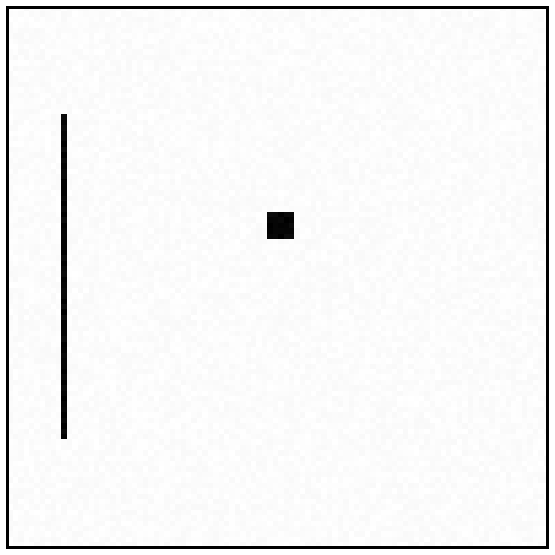
\includegraphics[width=.5in]{position_common_scale.pdf}} & \makecell[tl]{\emph{Position Common Scale}\\ \begin{tabular}{ccccccc}
%
%\end{tabular}} \\
%
%	\midrule
%	\raisebox{-.85\height}{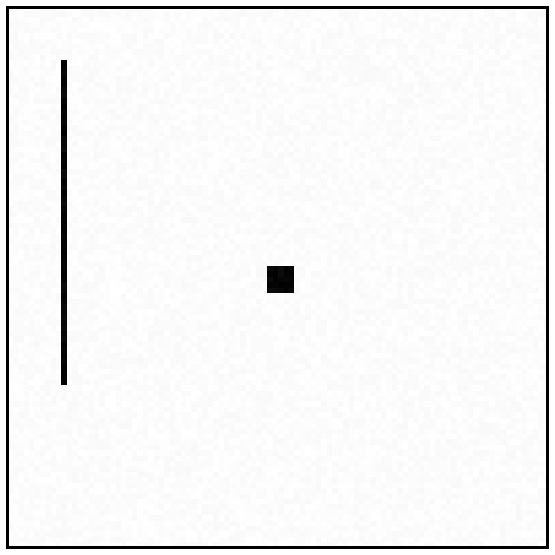
\includegraphics[width=.5in]{position_non_aligned_scale.pdf}} & \makecell[tl]{\emph{Position Non-Aligned Scale}\\~~~Position Y\\~~~+ Position X \\~~~+ Spot Size \\} &~& \makecell[tr]{~\\ $600$ \\ $36,000$ \\ $216,000$}\\
%
%	\midrule
%	\raisebox{-.95\height}{
\includegraphics[width=.5in]{length.pdf}} & \makecell[tl]{\emph{Length}\\~~~Length\\~~~+ Position Y \\~~~+ Position X \\~~~+ Width} &~& \makecell[tr]{ ~\\$60$ \\ $2,400$ \\ $144,000$\\$864,000$}\\
%
%	\midrule
%	\raisebox{-.85\height}{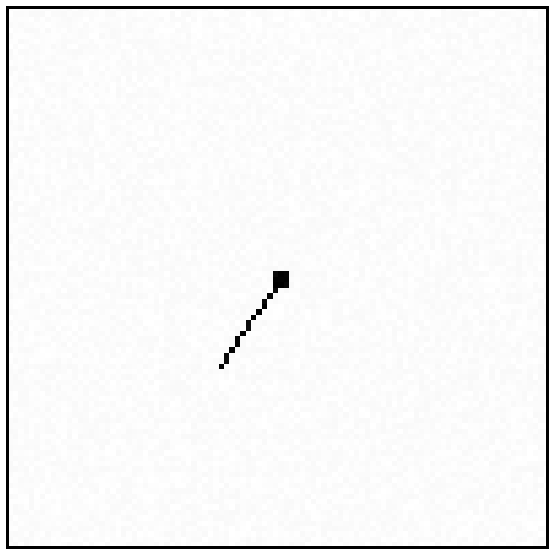
\includegraphics[width=.5in]{direction.pdf}} & \makecell[tl]{\emph{Direction}\\~~~Angle\\~~~+ Position Y \\~~~+ Position X} &~& \makecell[tr]{ ~\\$360$ \\ $21,600$ \\ $1,296,000$}\\
%
%	\midrule
%	\raisebox{-.85\height}{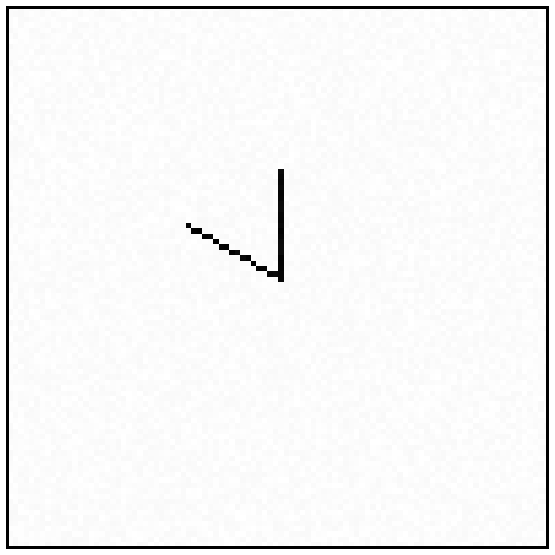
\includegraphics[width=.5in]{angle.pdf}} & \makecell[tl]{\emph{Angle}\\~~~Angle\\~~~+ Position Y \\~~~+ Position X} &~& \makecell[tr]{ ~\\$90$ \\ $5,400$ \\ $324,000$}\\
%
%	\midrule
%	\raisebox{-.85\height}{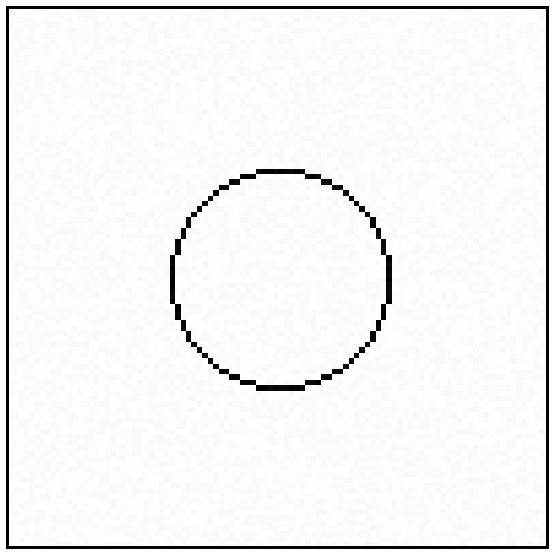
\includegraphics[width=.5in]{area.pdf}} & \makecell[tl]{\emph{Area}\\~~~Radius\\~~~+ Position Y \\~~~+ Position X} &~& \makecell[tr]{ ~\\$40$ \\ $800$ \\ $16,000$}\\
%
%	\midrule
%	\raisebox{-.85\height}{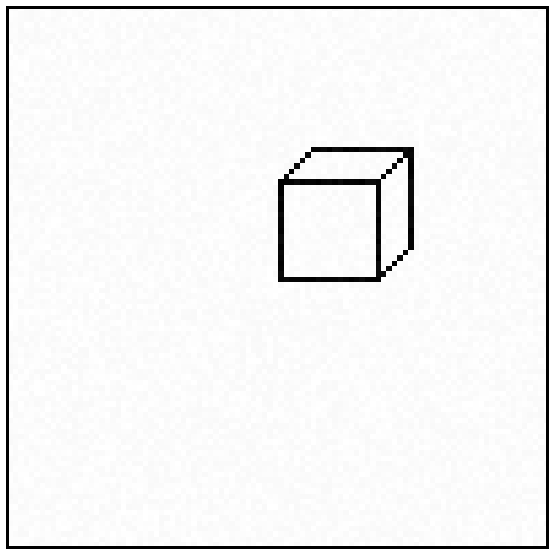
\includegraphics[width=.5in]{volume.pdf}} & \makecell[tl]{\emph{Volume}\\~~~Cube Sidelength\\~~~+ Position Y \\~~~+ Position X} &~& \makecell[tr]{ ~\\$20$ \\ $400$ \\ $8,000$}\\
%	
%	\midrule
%	\raisebox{-.85\height}{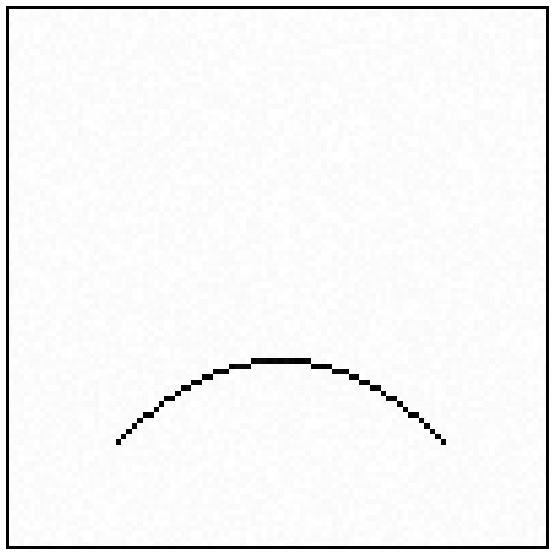
\includegraphics[width=.5in]{curvature.pdf}} & \makecell[tl]{\emph{Curvature}\\~~~Midpoint Curvature\\~~~+ Position Y \\~~~+ Position X} &~& \makecell[tr]{ ~\\$80$ \\ $1,600$ \\ $64,000$}\\	
%
%	\midrule
%	\raisebox{-.85\height}{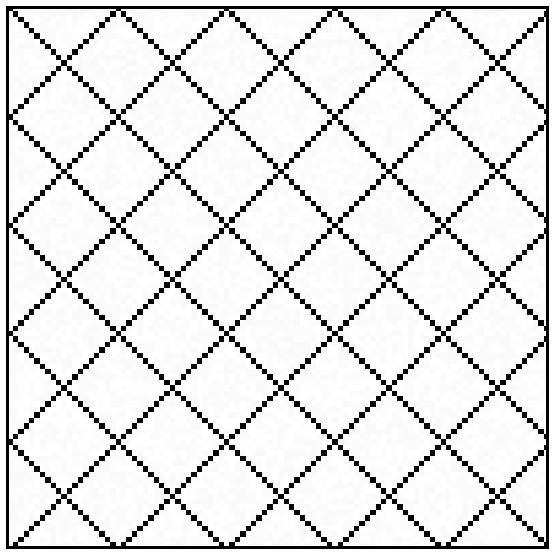
\includegraphics[width=.5in]{shading.pdf}} & \makecell[tl]{\emph{Shading}\\~~~Density\\~~~+ Position Y \\~~~+ Position X} &~& \makecell[tr]{ ~\\$100$ \\ $2,000$ \\ $40,000$}\\	

	\bottomrule
\end{tabular}
}
\label{tab:ranking}
\end{table}

\begin{figure}[!ht]
	\centering
	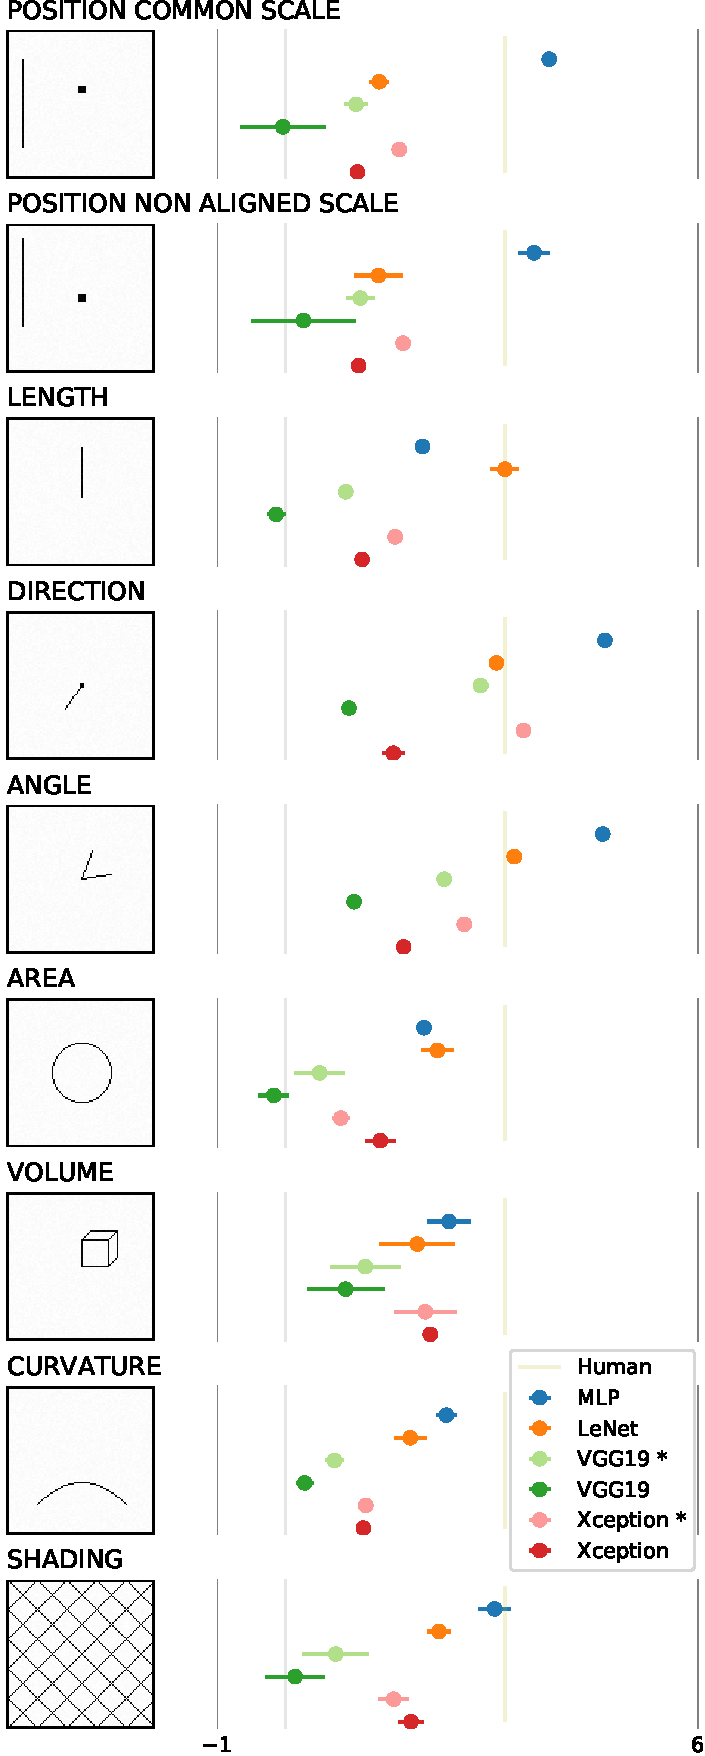
\includegraphics[width=.8\linewidth]{figure1_slim_only_last.pdf}
%	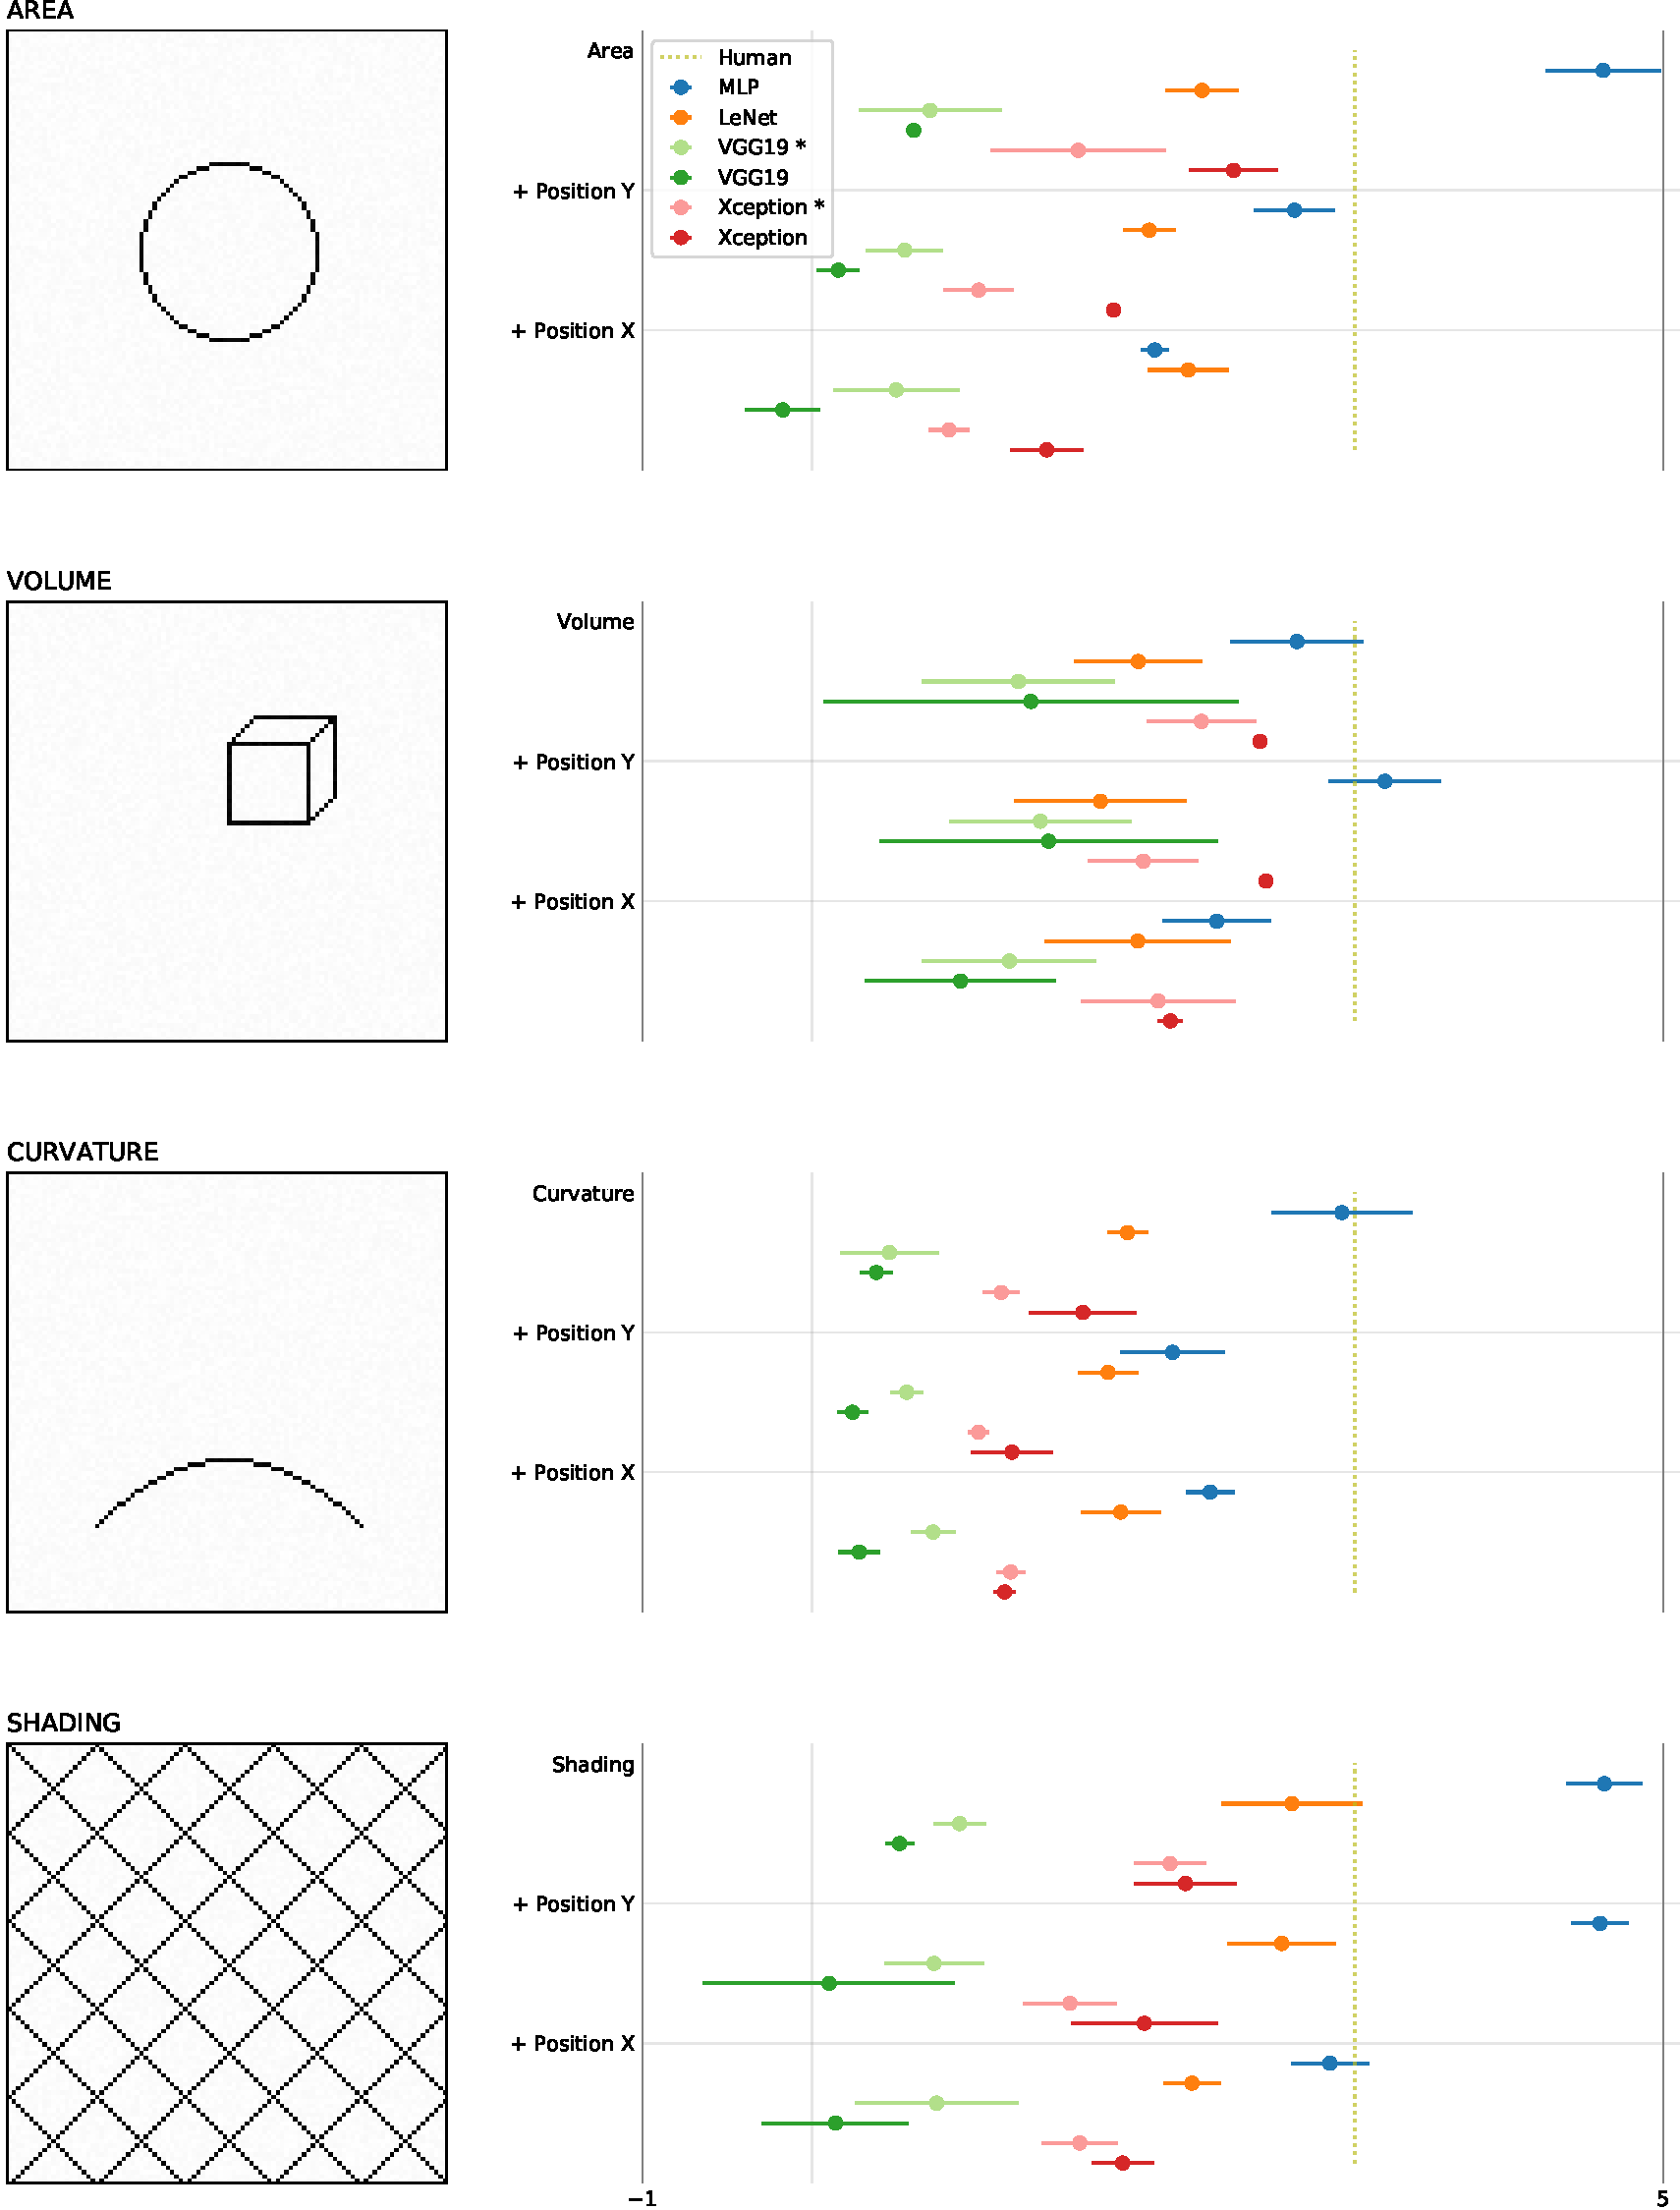
\includegraphics[width=0.48\linewidth]{figure1_slim_right.pdf}
	\caption{\textbf{Computational results of Elementary Perceptual Tasks experiment.} Log absolute error means and 95\% confidence intervals for computed perception of different classifiers on the \emph{elementary perceptual tasks} introduced by Cleveland and McGill 1984~\cite{cleveland_mcgill}. We test the performance of a Multi-layer Perceptron (MLP), the LeNet Convolutional Neural Network, as well as feature generation using the VGG19 and Xception networks on the most complex parametrizations. The * indicates networks which use ImageNet weights. We also compare against an approximate human baseline of $9\%$ error reported by Cleveland and McGill.}
	\label{fig:figure1_results}
\end{figure}

\noindent{\textbf{Cross-classifier Variability and Network Generalizability.}} We measure regression performance across classifiers trained on the different parameterizations of the elementary perceptual tasks. Looking at the results in Fig.~\ref{fig:cross_network}, we can observe that even slight variations of an encoding such as added translation in Y or X drastically increases the error. We think that the networks are not really learning concepts of perception but rather learn the variation of pixel values.

\begin{figure}[!ht]
	\centering
	  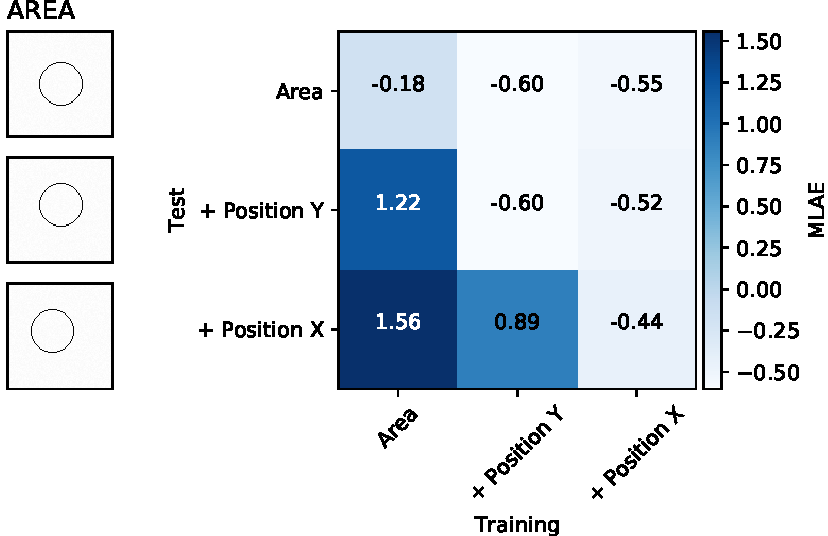
\includegraphics[width=.75\linewidth]{cross_network_small_VGG19_area.pdf}
	  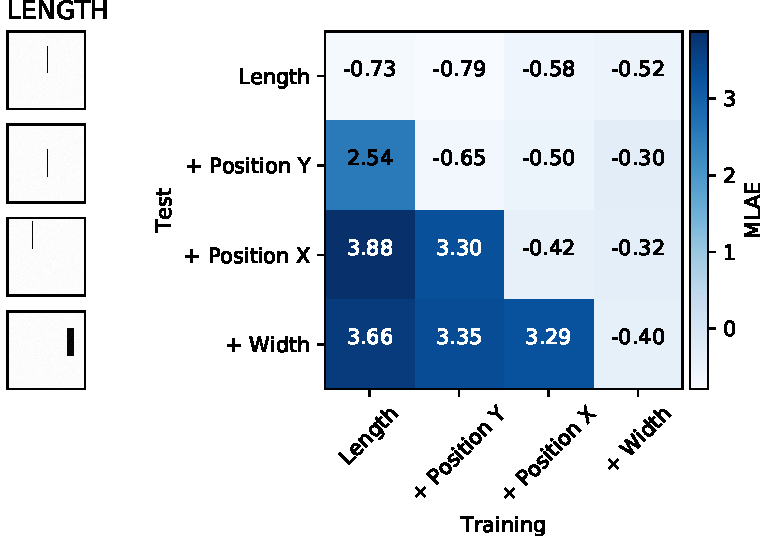
\includegraphics[width=.75\linewidth]{cross_network_small_VGG19_length.pdf}
	  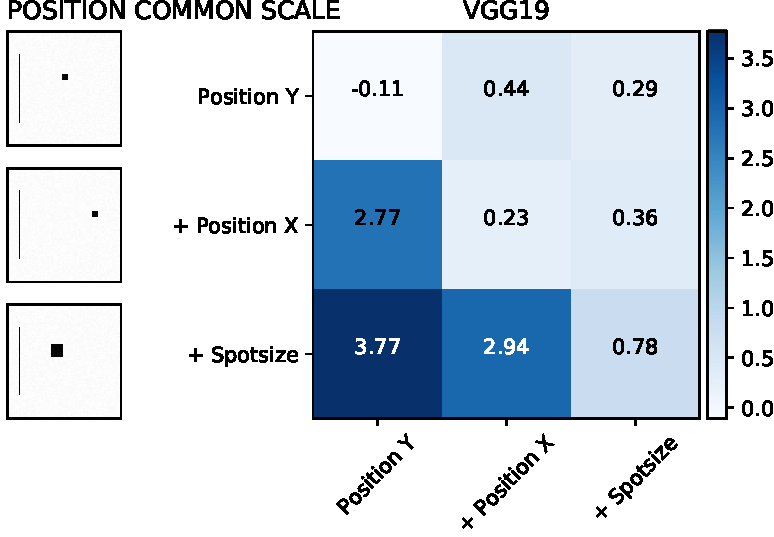
\includegraphics[width=.75\linewidth]{cross_network_small_VGG19_position_common_scale.pdf}
	  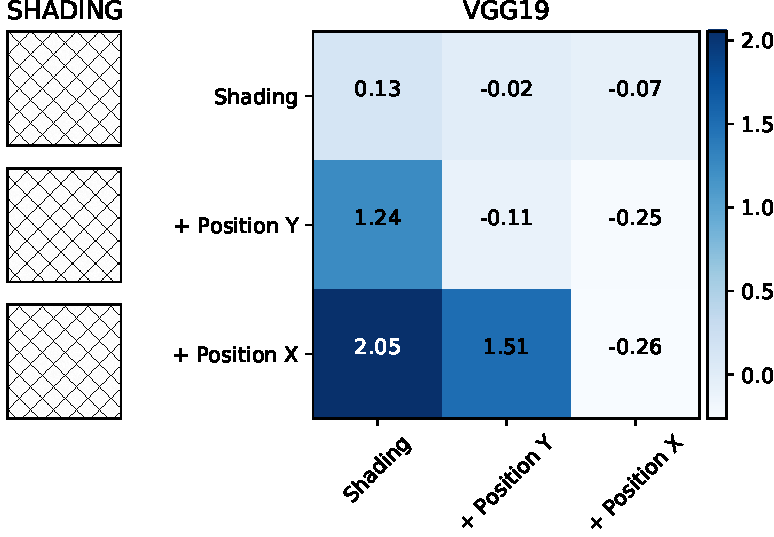
\includegraphics[width=.75\linewidth]{cross_network_small_VGG19_shading.pdf}
  \caption{\textbf{Cross-classifier variability for perceptual tasks.} We use predictions of the VGG19 network trained on different parametrizations of \emph{area}, \emph{length}, \emph{position common scale}, and \emph{shading}. These are the top 4 encodings in the ranking for this network. We measure the mean logistic absolute error (MLAE) -- the lower score, the better. Regressors trained on stimuli with variable position can generalize even if the axis of translation varies. However, if they are trained on fixed positions of the stimuli they are not able to measure translated encodings.}
	\label{fig:cross_network}
\end{figure}

